% Intended LaTeX compiler: pdflatex
\documentclass[10pt,a4paper,UTF8]{article}
\usepackage{zclorg}
\author{张朝龙}
\date{}
\title{练习:矩阵}
\hypersetup{
 pdfauthor={张朝龙},
 pdftitle={练习:矩阵},
 pdfkeywords={},
 pdfsubject={},
 pdfcreator={Emacs 25.0.50.1 (Org mode 9.0.5)}, 
 pdflang={English}}
\begin{document}

\maketitle
\tableofcontents
\titlepic{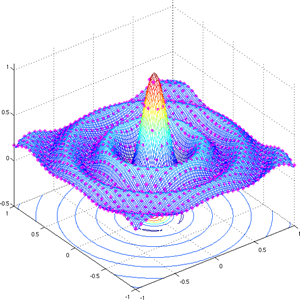
\includegraphics[scale=0.25]{../../img/sinc.PNG}}
本章的题目都不难,只要紧扣线性映射矩阵的定义和矩阵加法,矩阵标量乘法,矩阵乘法的定义即可轻松完成所有题目。为节省时间,最后几个题目略去不提。

\section{3.C.1}
\label{sec:orgd0a8bba}


\begin{problem}
设\(V\)和\(W\)都是有限维的,\(T\in \mathcal{L}(V,W)\),证明对于\(V\)和\(W\)的任意基,\(T\)的矩阵都至少有\(\dim rangeT\)个非零元
\end{problem}

\begin{answer}
首先我们知道\(rangeT\)中一定有\(\dim rangeT\)个线性无关的向量\(u_{1},u_{2},\ldots ,u_{m}\), \(m = \dim rangeT\)。\(rangeT\)就是由这些向量张成的子空间。
\end{answer}
\section{3.C.2}
\label{sec:org988b892}


\begin{problem}
设\(D\in \mathcal{L}( \mathcal{P}_{3}( \mathbf{R}),\mathcal{P}_{2}(\mathbf{R}))\)是微分映射\(Dp = p^{'}\),求\(\mathcal{P}_{3}( \mathbf{R})\)的一个基和\(\mathcal{P}_{2}(R)\)的一个基,使得\(D\) 关于这些基的矩阵为:
\begin{equation*}
\begin{bmatrix}
1 & 0 & 0 & 0 \\
0 & 1 & 0 & 0 \\
0 & 0 & 1 & 0
\end{bmatrix}
\end{equation*}
\end{problem}

\begin{answer}
这里在重复一下根据线性映射定义矩阵的过程。假设\(V\)的基是\(v_{1},\ldots ,v_{n}\),\(W\)的基是\(w_{1},\ldots ,w_{m}\),有线性映射\(T\in \mathcal{L}(V,W)\),则\(T\)关于\(V\)和\(W\)的两个基定义的矩阵是\(A\),则有
\begin{equation}
\label{eq:1}
Tv_{k} = A_{1,k}w_{1} + \ldots + A_{m,k}w_{m}
\end{equation}

对于题目中给定的矩阵。我们有:
\begin{eqnarray}
\label{eq:2}
Tv_{1}&=& w_{1} \\
Tv_{2}&=& w_{2} \\
Tv_{3}&=& w_{3} \\
Tv_{4}&=& 0
\end{eqnarray}
一个可能的组合是:\(V\)的基为\(\{x,\frac{x^{2}}{2},\frac{x^{3}}{3},1 \}\),\(W\)的基为\(1,x,x^{2}\) 。

显然有:
\begin{eqnarray*}
T(x)&=& 1\\
T(x^{2}/2)&=& x\\
T(x^{3}/3)&=& x^{2}\\
T(1) &=& 0
\end{eqnarray*}
\end{answer}
\section{3.C.3}
\label{sec:org558579c}


\begin{problem}
设\(V\)和\(W\)都是有限维的,\(T\in \mathcal{L}(V,W)\).证明存在\(V\)的一个基和\(W\)的一个基使得关于这些基,\(\mathcal{M}(T)\)除了第\(j\)行第\(j\)列\(1\leq j \leq \dim range T\)的元素意外,其余元素都为\(0\)
\end{problem}

\begin{answer}
根据线性映射矩阵定义,\(\mathcal{M}(T)\)的行是\(rangeT\)基的大小。我们定义线性映射:
\begin{equation}
\label{eq:3}
Tv_{k} = w_{k},k =1,\ldots ,\dim range T
\end{equation}
\begin{equation}
\label{eq:4}
Tv_{k} = 0, k=\dim range T + 1 ,\ldots ,\dim V
\end{equation}
这个映射对应的矩阵就是题目中所描述的矩阵。

在证明过程中,采用的思路和证明线性映射基本定理相同。
\end{answer}
\section{3.C.4}
\label{sec:org76ae909}


\begin{problem}
设\(v_{1},\ldots ,v_{m}\)是\(V\)的基,且\(W\)是有限维的。设\(T\in \mathcal{L}(V,W)\)。证明存在\(W\)的一个基\(w_{1},\ldots ,w_{n}\)使得在\(T\)关于基\(v_{1},\ldots ,v_{m}\)和\(w_{1},\ldots ,w_{n}\)的矩阵\(\mathcal{M}(T)\)中,除了第一行第一列的元素可能为1之外,第一列的其余元素均为0.
\end{problem}

\begin{answer}
存在映射:\(T\in (V,W)\)满足:
\begin{eqnarray*}
Tv_{1}&=&w_{1} \\
Tv_{2}&=&w_{1} + w_{2} \\
\vdots && \vdots \\
Tv_{n} &=& w_{n-1} + w_{n}
\end{eqnarray*}
\end{answer}
\section{3.C.5}
\label{sec:org62e4bad}


\begin{problem}
设\(w_{1},\ldots ,w_{n}\)是\(W\)的一个基,且\(V\)是有限维的。设\(T\in \mathcal{L}(V,W)\)。证明存在\(V\)的一个基\(v_{1},\ldots ,v_{m}\)使得,在\(T\)关于\(v_{1},\ldots ,v_{m}\)和\(w_{1},\ldots ,w_{n}\)的矩阵\(\mathcal{M}(T)\)中,除了第一行第一列的元素可能为1之外,第一行的其余元素均为0。
\end{problem}

\begin{answer}
这个题目的证明和3.C.4类似。略。做这样的题目的时候最好把从线性映射定义矩阵的过程给默想一遍。
\end{answer}

\section{3.C.6}
\label{sec:org621f3b5}


\begin{problem}
设\(V\)和\(W\)都是有限维的,\(T\in \mathcal{L}(V,W)\) 证明\(\dim rangeT = 1\)当且仅当\(V\)和\(W\)各有一个基使得关于这些基\(\mathcal{M}(T)\)的所有元素都是1.
\end{problem}

\begin{answer}
我们先从当\(V\)和\(W\)各有一个基使得关于这些基\(\mathcal{M}(T)\)的所有元素都是1导出\(\dim rangeT = 1\)

根据线性映射基本定理的证明过程,我们知道\(V\)的基中存在一个线性无关组\(u_{1},\ldots ,u_{n}\)张成了\(nullT\),而另外一些线性无关向量\(v_{1},\ldots ,v_{m}\)是基于\(u_{1},\ldots ,u_{n}\)扩展而来的。


假设 \(w_{1},\ldots ,w_{p}\)是\(W\)的一个基,定义线性映射:
\begin{eqnarray*}
Tv_{1}&=&w_{1} + \ldots + w_{p} \\
\vdots && \vdots \\
Tv_{n}&=&w_{1} + \ldots + w_{p} 
\end{eqnarray*}

这个线性映射满足\(\dim range T = 1\)

接下来我们证明另外一方面.因为\(\dim rangeT = 1\),我们有以上定义的线性映射满足\(\mathcal{M}(T)\)的所有元素都是1。

证明这个命题,主要还是采用线性映射基本定理中的方法。
\end{answer}
\section{3.C.7}
\label{sec:org27a05b8}


\begin{problem}
验证 3.36
\end{problem}

\begin{answer}
从线性映射的矩阵定义出发。略。
\end{answer}
\section{3.C.8}
\label{sec:org03c8ab7}


\begin{problem}
验证3.38
\end{problem}

\begin{answer}
从线性映射的矩阵定义出发。
\end{answer}

\section{3.C.9}
\label{sec:org0dbf459}


\begin{problem}
证明3.52
\end{problem}

\begin{answer}
从矩阵乘法定义出发。假设
\begin{equation}
\label{eq:5}
A = 
\begin{bmatrix}
A_{1,1} & \ldots & A_{1,n} \\
\vdots & \ddots & \vdots \\
A_{m,1} & \ldots & A_{m,n}
\end{bmatrix}
\end{equation}
则\(Ac\)是一个\(m\times 1\)的列向量。并且有:
\begin{equation}
\label{eq:6}
Ac =
\begin{bmatrix}
\sum_{i=1}^{n}A_{1,i}c_{i} \\
\sum_{i=1}^{n}A_{2,i}c_{i} \\
\vdots \\
\sum_{i=1}^{n}A_{mi}c_{i} \\
\end{bmatrix}
\end{equation}

通过对上式右端展开,得:
\begin{equation*}
Ac =
\begin{bmatrix}
\sum_{i=1}^{n}A_{1,i}c_{i} \\
\sum_{i=1}^{n}A_{2,i}c_{i} \\
\vdots \\
\sum_{i=1}^{n}A_{mi}c_{i} 
\end{bmatrix}
= 
c_{1} 
\begin{bmatrix}
A_{1,1} \\ A_{2,1} \\ \vdots \\A_{m,1}
\end{bmatrix}
+
c_{2} 
\begin{bmatrix}
A_{1,2} \\ A_{2,2} \\ \vdots \\A_{m,2}
\end{bmatrix}
+ 
\ldots 
+
c_{n} 
\begin{bmatrix}
A_{1,n} \\ A_{2,n} \\ \vdots \\A_{m,n}
\end{bmatrix}
\end{equation*}
\end{answer}

\section{3.C.10}
\label{sec:org28aed9e}


\begin{problem}
设\(A\)是\(m\times n\)矩阵,\(C\)是\(n\times p\)矩阵。证明对于\(1\leq j \leq m\) \((AC)_{j,\cdot} = A_{j,\cdot}C\)

也就是说,证明\(AC\)的第\(j\)行等于\(A\)的第\(j\)行乘以\(C\)
\end{problem}

\begin{answer}
略去证明。

在学习MIT Strang教授的线性代数时掌握这种观点。\(AC\)的每一行是\(C\)的行向量的线性组合,线性组合系数是\(A\)对应的行的元素。
\end{answer}

\section{3.C.11}
\label{sec:org9664662}


\begin{problem}
设\(a=(a_{1} \quad \ldots \quad a_{n})\)是\(1\times n\)矩阵,\(C\)是\(n\times p\)矩阵。证明\[aC = a_{1}C_{1,\cdot} + \ldots + a_{n}C_{n,\cdot}\]
\end{problem}

\begin{answer}
此题是3.C.10 的特例。
\end{answer}
\end{document}
